\chapter{Future Tenses}

Future tenses describe actions or events that will happen. They help you express plans, predictions, schedules, and actions that will be completed at a later time. Mastering these forms improves clarity and effectiveness in everyday communication.

\section{Going To vs Will for Future Plans and Predictions}

Two common ways to express future actions in English are using ``going to'' and ``will''. Understanding the difference between these two forms is essential for effective communication.

\begin{tcolorbox}[colback=blue!5, colframe=blue!30, title=Future Tense Comparison]

	\textbf{``Going to''} is used for plans or intentions that have already been decided before the moment of speaking. 

	\textit{Example.} ``I am going to visit my grandparents next weekend.'' 

This indicates a pre-planned action.

\vspace{0.5cm}

	\textbf{``Will''} is used for spontaneous decisions made at the moment of speaking or for predictions about the future. 

	\textit{Example.} ``I will help you with your homework.'' 

This indicates a decision made on the spot or a prediction based on current knowledge.

\end{tcolorbox}



\section{Future Simple (Will)}

The future simple with ``will'' expresses decisions made at the moment of speaking, general predictions, promises, offers, and future facts.

\begin{tcolorbox}[colback=purple!5, colframe=purple!30, title=Future Simple (Will)]
	\textbf{Structure:}
\begin{itemize}
    \item Affirmative: Subject + will + base verb
    \item Negative: Subject + will not (won't) + base verb
    \item Interrogative: Will + subject + base verb?
\end{itemize}
	\textbf{Examples:}
\begin{itemize}
    \item ``I'll call you later.'' (decision now)
    \item ``It will rain tomorrow.'' (prediction)
    \item ``We won't be late.'' (negative)
    \item ``Will you help me?'' (offer/request)
\end{itemize}
\end{tcolorbox}

\section{Present Continuous for Future Arrangements}

The present continuous is often used to talk about fixed plans and arrangements, usually when a time is specified.

\begin{tcolorbox}[colback=orange!5, colframe=orange!30, title=Present Continuous (Future Arrangements)]
	\textbf{Structure:}
\begin{itemize}
    \item Affirmative: Subject + am/is/are + verb\,–ing + time reference
    \item Negative: Subject + am/is/are not + verb\,–ing + time reference
    \item Interrogative: Am/Is/Are + subject + verb\,–ing + time reference?
\end{itemize}
	\textbf{Examples:}
\begin{itemize}
    \item ``I'm meeting the manager at 3 p.m.''
    \item ``She's flying to Madrid next Monday.''
    \item ``Are you having dinner with them tonight?''
\end{itemize}
\end{tcolorbox}


\section{Future Perfect Tense}

The future perfect tense is used to describe an action that will be completed before a specific point in the future. It is formed using ``will have'' followed by the past participle of the verb.

\begin{tcolorbox}[colback=green!5, colframe=green!30, title=Future Perfect Tense]
\textbf{Structure:}
\begin{itemize}
    \item Affirmative: Subject + will have + past participle
    \item Negative: Subject + will not have + past participle
    \item Interrogative: Will + subject + have + past participle?
\end{itemize}
\end{tcolorbox}

	extit{Example.} ``By next year, I will have completed my degree.''


\section{Future Continuous Tense}

The future continuous tense is used to describe actions that will be in progress at a specific time in the future. It is formed using ``will be'' followed by the present participle (verb + -ing).

\begin{tcolorbox}[colback=yellow!5, colframe=yellow!30, title=Future Continuous Tense]
\textbf{Structure:}
\begin{itemize}
    \item Affirmative: Subject + will be + verb\,–ing
    \item Negative: Subject + will not be + verb\,–ing
    \item Interrogative: Will + subject + be + verb\,–ing?
\end{itemize}
\end{tcolorbox}

	extit{Example.} ``This time tomorrow, I will be flying to Paris.''

\section{Future Perfect Continuous}

The future perfect continuous focuses on the duration of an activity up to a point in the future. It is formed with ``will have been'' + verb\,–ing.

\begin{tcolorbox}[colback=teal!5, colframe=teal!30, title=Future Perfect Continuous]
	\textbf{Structure:}
\begin{itemize}
    \item Affirmative: Subject + will have been + verb\,–ing
    \item Negative: Subject + will not have been + verb\,–ing
    \item Interrogative: Will + subject + have been + verb\,–ing?
\end{itemize}
	\textbf{Example:}
\begin{itemize}
    \item ``By noon, they will have been working for five hours.''
\end{itemize}
\end{tcolorbox}

\section{Time Expressions}

Common future time markers help identify the correct tense: \textit{tomorrow, next week/month/year, in two days, soon, later, this evening, by 2026, at 5 p.m., on Monday}.

\section{Common Mistakes with Future Tenses}

Learners often confuse the use of ``going to'' and ``will''. Here are some common mistakes to avoid:

\begin{itemize}
    \item Using ``will'' for planned actions instead of ``going to''.
    \item Confusing the future perfect with the future continuous.
    \item Omitting the past participle after ``will have'' in the future perfect.
\end{itemize}

\section{Practice Exercises}

	extbf{Exercise 1: Complete with the correct future form (``will'', ``going to'', future continuous, or future perfect).}

1. I \rule{2.5cm}{0.4pt} (go) to the store tomorrow.
2. By next month, she \rule{2.5cm}{0.4pt} (finish) her project.
3. This time next week, we \rule{2.5cm}{0.4pt} (travel) to Italy.

	extbf{Exercise 2: Correct the mistakes in the following sentences.}

1. I will going to the party tonight.
2. They will have complete the report by Friday.

\section{Conclusion}

Using future forms accurately lets you describe plans, make predictions, talk about schedules, and highlight completed actions by a future time. Practise choosing between ``will'' (decisions/predictions), ``going to'' (plans/intentions), the present continuous (arrangements), the future continuous (in-progress actions at a future time), the future perfect (completed by a future point), and the future perfect continuous (duration up to a future point).

\section{Summary}
Use ``going to'' for planned actions; ``will'' for spontaneous decisions, promises, and predictions; the \textit{present continuous} for fixed arrangements; the \textit{future continuous} for actions in progress at a future time; the \textit{future perfect} for actions completed before a specific future time; and the \textit{future perfect continuous} to emphasize duration up to a future point.


\subsection{Timeline Diagram}

\begin{figure}[H]
    \centering
    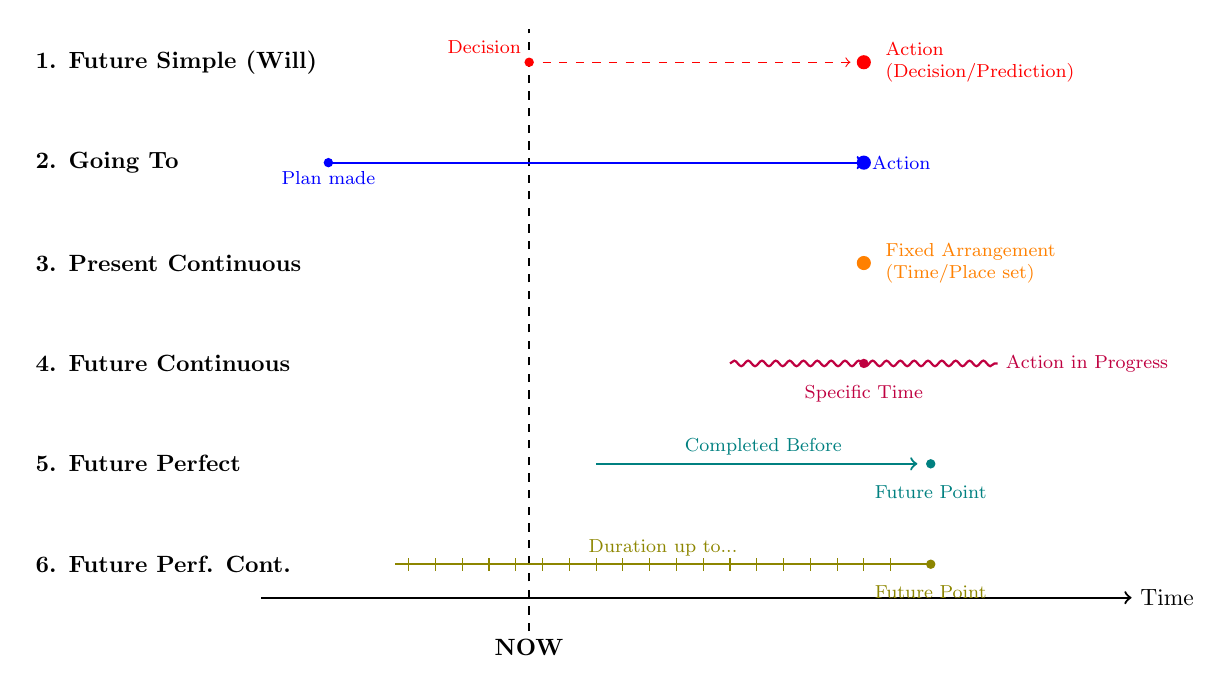
\begin{tikzpicture}[scale=0.85, transform shape]
        % Timeline axis
        \draw[->, thick] (-4,0) -- (9,0) node[right] {Time};
        
        % Now marker
        \draw[thick, dashed] (0, -0.5) -- (0, 8.5);
        \node[below] at (0, -0.5) {\textbf{NOW}};

        % 1. Future Simple (Will)
        \node[anchor=west] at (-7.5, 8) {\textbf{1. Future Simple (Will)}};
        \fill[red] (5, 8) circle (3pt);
        \node[right, red, align=left, font=\footnotesize] at (5.2, 8) {Action\\(Decision/Prediction)};
        \draw[->, red, dashed] (0.2, 8) -- (4.8, 8);
        \fill[red] (0, 8) circle (2pt) node[above left, font=\footnotesize] {Decision};

        % 2. Going To
        \node[anchor=west] at (-7.5, 6.5) {\textbf{2. Going To}};
        \draw[blue, thick, ->] (-3, 6.5) -- (5, 6.5);
        \fill[blue] (-3, 6.5) circle (2pt) node[below, font=\footnotesize] {Plan made};
        \fill[blue] (5, 6.5) circle (3pt) node[right, font=\footnotesize] {Action};

        % 3. Present Continuous
        \node[anchor=west] at (-7.5, 5) {\textbf{3. Present Continuous}};
        \fill[orange] (5, 5) circle (3pt);
        \node[right, orange, align=left, font=\footnotesize] at (5.2, 5) {Fixed Arrangement\\(Time/Place set)};

        % 4. Future Continuous
        \node[anchor=west] at (-7.5, 3.5) {\textbf{4. Future Continuous}};
        \draw[decorate, decoration={snake, amplitude=1pt, segment length=5pt}, thick, purple] (3, 3.5) -- (7, 3.5);
        \fill[purple] (5, 3.5) circle (2pt);
        \node[below, purple, font=\footnotesize] at (5, 3.3) {Specific Time};
        \node[right, purple, font=\footnotesize] at (7, 3.5) {Action in Progress};

        % 5. Future Perfect
        \node[anchor=west] at (-7.5, 2) {\textbf{5. Future Perfect}};
        \draw[->, thick, teal] (1, 2) -- (5.8, 2);
        \fill[teal] (6, 2) circle (2pt);
        \node[below, teal, font=\footnotesize] at (6, 1.8) {Future Point};
        \node[above, teal, font=\footnotesize] at (3.5, 2) {Completed Before};

        % 6. Future Perfect Continuous
        \node[anchor=west] at (-7.5, 0.5) {\textbf{6. Future Perf. Cont.}};
        \draw[thick, olive] (-2, 0.5) -- (6, 0.5);
        \foreach \x in {-1.8, -1.4, ..., 5.8} \draw[olive] (\x, 0.4) -- (\x, 0.6);
        \fill[olive] (6, 0.5) circle (2pt);
        \node[below, olive, font=\footnotesize] at (6, 0.3) {Future Point};
        \node[above, olive, font=\footnotesize] at (2, 0.5) {Duration up to...};

    \end{tikzpicture}
    \caption{Visualizing Future Tenses}
    \label{fig:future_tenses}
\end{figure}
